\chapter{Internet das Coisas Aplicações em Mobilidade Urbana e Saúde}
\label{chap:cap1}
Internet das coisas, conhecido também como IoT, sigla que em inglês significa \textit{Internet Of Things}, originou-se através de Kevin Ashton que em 1999 realizou uma apresentação na empresa  Procter \& Gamble (P\&G), quando falava em se etiquetar eletronicamente os produtos da empresa através do uso de Identificador de Rádio Frequência (RFID), assunto que era recente na época. Desde então este paradigma tem sido muito discutido, principalmente no contexto atual, em que é possível notar um crescimento exponencial de tecnologias desenvolvidas neste sentido, como é mostrado na figura \ref{fig:graficoIot2011-2025} que apresenta o aumento no uso de IoT mundialmente, fazendo uma estimativa até o ano de 2025.\cite{historiaiot} 

\begin{figure}[htb]
\caption{\label{fig:graficoIot2011-2025}Gráfico de crescimento do IoT entre os anos de 2011 a 2025}
\begin{center}
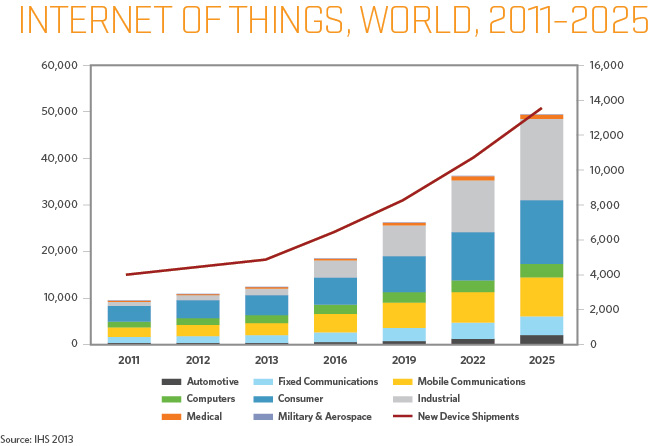
\includegraphics[scale=0.6]{graficoIot2011-2025}
\end{center}
\legend{Fonte: IHS 2013}
\end{figure}

O aumento do uso de IoT se dá pelo avanço da tecnologia em diversas áreas, fazendo com que objetos se relacionem entre si de forma autônoma, a fim de gerar maior facilidade na realização de tarefas humanas, além de fornecer uma grande quantidade de dados relevantes que auxiliam na tomada de decisões. Apesar da autonomia vista entre os objetos deste sistema, quem tem o total poder é o usuário final, podendo ele estar controlando tudo pelo seu smartphone ou por uma central de gerenciamento.\cite{presser2011}

\begin{citacao}
Quando os objetos podem sentir o ambiente e se comunicar, eles se tornam ferramentas poderosas para entender coisas complexas e responder a elas com eficiência. Embora tais objetos inteligentes possam interagir com humanos, é mais provável que interajam ainda mais entre si automaticamente, sem intervenção humana atualizando-se com as tarefas do dia.\cite[p. 2]{presser2011}
\end{citacao}

\section{O que é IoT?}
\label{sec:oqueeiot}











%\autoref{chap:cap1}
% ---
%\section{Aliquam vestibulum fringilla lorem}
%\lipsum[2]
%\subsection{Subsessão cap 1}
%\lipsum[2]
%\chapter{Capitulo Segundo}
%\lipsum[2]